\documentclass{report}
\usepackage{graphicx}
\usepackage[ngerman]{babel}
\usepackage[utf8]{inputenc}
\usepackage[T1]{fontenc}
\usepackage{hyperref}
\usepackage{csquotes}
\usepackage[a4paper]{geometry}
\usepackage[
    backend=biber,
    style=apa,
    sortlocale=de_DE,
    natbib=true,
    url=false,
    doi=false,
    sortcites=true,
    sorting=nyt,
    isbn=false,
    hyperref=true,
    backref=false,
    giveninits=false,
    eprint=false]{biblatex}
\addbibresource{../references/bibliography.bib}


\title{Data Ethics and AI}
\author{Nikolay Voropayev}
\date{\today}


\begin{document}

\maketitle

\abstract{
    In diesem Dokument wird grob erklaert wie KI funktioniert, es werden die Gefahren von KI analysiert, logisch behandelt und schlussfolgerungen gezogen, welchen beweisen sollen, dass: 
    \begin{enumerate}
        \item KI is nicht wirklich intelligent
        \item KI wird uns nicht ausloeschen wie in der \hyperlink{https://en.wikipedia.org/wiki/The_Terminator}{Terminator-Franchise}.
        \item KI soll nicht nur in den haenden von Big-Tech Firmen ueberlassen werden, sondern sollte \hyperlink{https://en.wikipedia.org/wiki/Open-source_software}{open-source} gehalten werden.
        \item Datenschutz im zusammenhang mit KI is umsomehr wichtig als normalerweise.
    \end{enumerate}
}

\tableofcontents

\chapter{Einleitung}
\section{Was is KI?}
KI steht fuer "Kuenstilche Intelligenz", jedoch sieht KI gar nicht so aus wie ein menschliches Gehirn, welches aus Milliarden von Neuronen besteht.
KI's bestehen aus sogennanten \hyperlink{https://www.ibm.com/topics/artificial-intelligence}{Neuralen Netzwerken}.
\begin{figure}[h]
    \centering 
    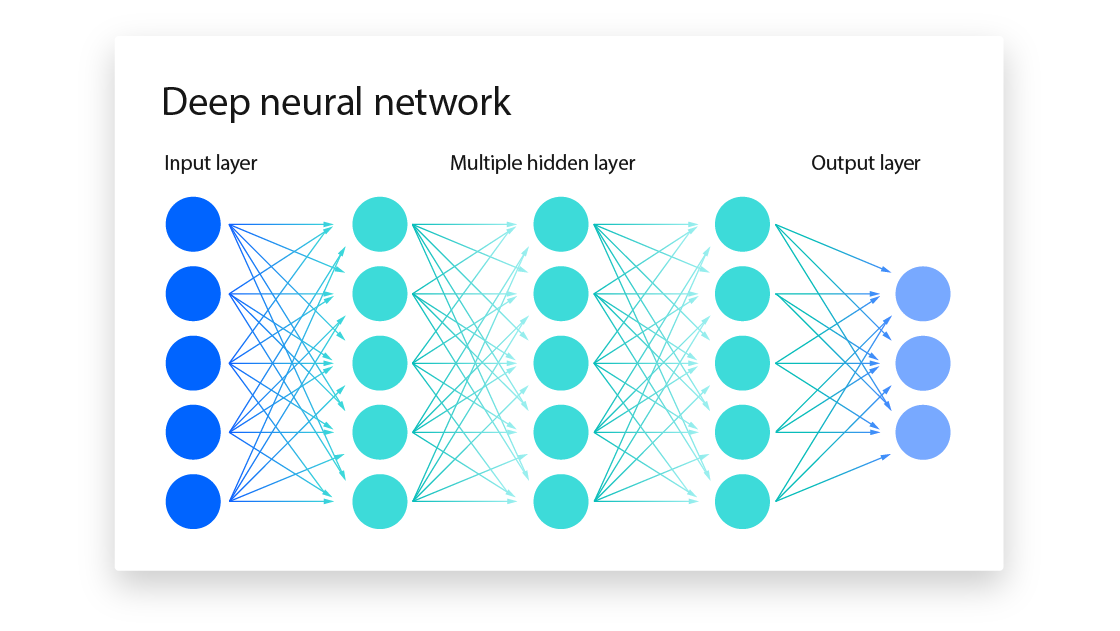
\includegraphics[width=1\textwidth]{NN-ibm.png} 
    \caption{Neurale-Netzwerk-Grafik, IBM}
    \label{fig:meme}
\end{figure}

Ich werde in dieser Arbeit nicht in die Mathematischen details eingehen, auch nicht den Unterschied zwischen KI und \hyperlink{https://www.ibm.com/topics/machine-learning}{"Machine Learning"} erklaeren, da dies fuer diese Arbeit nicht besdonders wichtig ist. Auch wie diese Neuralen Netzwerke funktionieren 
wird auf der \hyperlink{https://www.ibm.com/topics/neural-networks}{IBM-website} gut erklaert.
\subsection{Was sind Neurale Netzwerke?}
Einfach erklaert, haben Neurale Netzwerke wie in der Abbildung Schichten. in jeder dieser Schichten gibt es Schnittpunkte. Wenn ein bestimmter Input einen Schnittpunkt aktiviert, sendet dieser einen bestimmten Output weiter. Wie stark dieser Output gewichtet ist, und wie er verarbeitet wird, haengt von dem Netzwerk ab.
Das wichtigste ist aber, dass man nicht wissen kann, was in diesen Netzwerken passiert, und warum ein bestimmter Input so wahrgenommen wird, wie er wird. Dies ist fuer spaeter wichtig.

Falls es schwer faellt, dies im Textformat zu verstehen, kann dieses \hyperlink{https://youtube.com/watch?v=p6CfR3Wpz7Y&t=390}{Video} dabei helfen.

\section{Was ist Datenschutz und warum ist es wichtig?}
Per \hyperlink{https://www.merriam-webster.com/dictionary/data}{mirriam-webster} sind Daten faktuelle Informationen.
Jedoch wenn wir von Daten im bezug auf Datenschutz sprechen, sind nicht einfach Statistiken zum Schokoladen-Konsum des Durchschnittlichen Schweizers, welches \hyperlink{https://de.statista.com/statistik/daten/studie/369440/umfrage/pro-kopf-konsum-von-schokolade-in-der-schweiz/}{ueber 10kg pro kopf pro jahr betraegt},
sondern es geht um Informationen, wie Lokationsdaten, die durch Bluetooth, WLAN oder Mobilfunknetze durch triangulation ausgerechnet werden koennen. Oder Kaufgewohnheiten durch die Ausgabensdaten der Kredikarten.
Viele solche Daten koennen aus anderen "herausgelesen" werden. Manche schlussfolgerungen zu schliessen ist es jedoch nicht moeglich fuer ein klassisches Computer-Programm.
\subsection{Warum ist Datenschutz wichtig?}
Dies ist ein sehr komplexes Thema und es gibt endlos Informationen dazu. Da es aber immer gut ist eine eigene Meinung zu bilden, werde ich einfach nur Beispiele bringen, warum Datenschutz wichtig sein kann.

Es gibt zalreiche vorfaelle bei denen zum Beispiel Versicherungs-Premien von Autofahrern in den Vereinigten Staaten hoeher wurde, weil sie stark gebremst haben, und wahrschleinlich ein KI entschieden hatte, dass dieser Autofaherer schlecht auto faheren kann. Auch wenn er in einer Situation bremste, in der er einen Unfall verhinderte.
\hyperlink{https://youtube.com/watch?v=aHhx8mMUV2o}{Video von CNN dazu.}

Aber dies ist nur eine Art, auf die unregulierter oder inkompetenter umgang mit Daten verherende Folgen hat, es gibt, wie ich schon erwaehnt habe, endlos solche beispiele.

Es gibt sehr viel Videos auf Youtube darueber, welche viel besse als ich es erklaeren koennte, zu diesem Thema erklaerungen bereitstellen, und dieser \hyperlink{https://youtube.com/channel/UCjr2bPAyPV7t35MvcgT3W8Q}{Youtube-Kanal} laesst fuer alle Informationen Quellen, dadurch ist es einfach die Informationen zu verarbeiten und sie koennen ueberprueft werden.
Ich wuerde empfehlen die unten gelisteten Videos anzuschauen.

\hyperlink{https://youtube.com/watch?v=WRalTWAFBY4}{Apple and Google contact tracing is a dystopian nightmare}

\hyperlink{https://youtube.com/watch?v=SrsCEbi5N7Y}{Google vs DuckDuckGo | Search engine manipulation, censorship and why you should switch}

\hyperlink{https://youtube.com/watch?v=vZBa5-wFAfQ}{Google will spy on you in physical stores – Can businesses really do anything?}

\hyperlink{https://youtube.com/watch?v=WX2SWUMt_fk}{Your Car Is a Better Spy than Facebook}

\hyperlink{https://youtube.com/watch?v=shpiVm1qpnw}{Don't use WhatsApp!}

\hyperlink{https://youtube.com/watch?v=vCRX0MZm2KI}{Your Keystrokes Are In The Cloud}
\newline
Falls man die Zeit hat, wuerde ich auch empfehlen, 1984 von George Orwell und 451 Fahrenheit von Ray Bredberry zu lesen, es sind sehr Spannende Buecher und sie haben mit der Thematik vieles gemeinsam.
Netuerlich ist dies alles nicht noetig, einfach um zu verstehen, warum Datenschutz wichtig ist, Die wichtigsten Quellen werden speater angegeben und werden auch markiert sein, das sie fuer ein verstaendnis noetig sind. Aber das wissen vom monumentalem Aussmass dieser Probleme ist nuetzlich. 
\chapter{KI, Daten und Ethik}
\section{KI und Daten}
Wie schon frueher erwaehnt, stellt KI neue moeglichkeiten for, Informationen zu verarbeiten. Ungluegcklicherweise bedeutet dies, dass eine KI Daten viel besser verarbeiten kann.
Die Social-Media-Platform \hyperlink{reddit.com}{Reddit} zum Beispiel verkauft alle Benutzer-Generierte Daten an \hyperlink{https://openai.com/}{OpenAI}, eine KI-firma, welche hauptsaechlich Microsoft gehoert.
Hier von der \hyperlink{https://openai.com/index/openai-and-reddit-partnership/}{offieziellen Website} von OpenAI. 
\newline
\newline
Technologien entwicklen sich sehr schnell, viel schneller als entsprechende Gesetze eingefuehrt werden koennen. So wurden zum Beispiel \hyperlink{https://en.wikipedia.org/wiki/Deepfake}{Deep-Fakes}, \hyperlink{https://edition.cnn.com/2024/05/16/tech/arup-deepfake-scam-loss-hong-kong-intl-hnk/index.html}{welche massive schaeden verursacht haben}, erst vor kurzen von Politikern als Problem anerkannt.
\newline
\newline
Das schockierendste ist, das es schon jetzt Socia-Credit-Scores gibt, die nicht von einem Diktaturstaat, sondern von Geschaeften, Banken und Versicherungsfirmen benutzt werden, um Kunden auf ihre "Wertigkeit" zu gradieren. All dies moeglich durch KI.
\hyperlink{https://youtube.com/watch?v=VUhKTngpd8c}{Dieses Video ist fuer das verstaendnis notwendig}
\newline
\newline
Es gibt auch eine grosse Luege, welche alle Big-Tech KI-Firmen immer wieder erzaehlen. Naehmlich sollte KI gefaehrlich sein, und es sollten nur bestimmte Firmen die erlaubnis haben, KI zu erstellen. Dies sollte durch Gesetze geregelt werden, die es schwer machen, ein eigenes, open-source KI-Modell selber herzustellen, und ja, dies ist \hyperlink{https://youtube.com/watch?v=188fipF-i5I}{moeglich}, und sogar realativ einfach, weswegen Big-Tech den lizenszugang sperren will.
\newline
Es gibt sogar ein \hyperlink{https://www.theguardian.com/technology/2023/may/05/google-engineer-open-source-technology-ai-openai-chatgpt}{Dokument}, welches von einem Google-Mitarbeiter geschrieben worde, in welchem beschreiben wird, wie open source modelle besser sind, als die, welche von Big-Tech erstellt werden und wie es unmoeglich ist, dagegen fair zu gewinnen.
\newline
\hyperlink{https://youtube.com/watch?v=5NUD7rdbCm8}{Dieses Video ist feur das verstaendnis notwendig}
\printbibliography

\end{document}
